\section{Experimental Evaluation}
\label{sec:evaluation}
\subsection{Experimental Setup}
We evaluate mean-token candidate scoring on MMLU~\cite{mmlu}, measuring
decision quality and complete-process throughput together. The RTX 4090
campaign comprises six pretrained models with CUDA and Vulkan and one
LoRA-adapted model with CUDA. Every full run covers the same 14,042 test
questions across 57 subjects, with reasoning disabled. A fixed subset supports
backend controls. Appendix~\ref{sec:reproducibility} specifies the protocol.

All thirteen RTX 4090 full-set runs and eighteen backend controls are complete
with mean-token scoring. The Arc A770 full-set and shared-prefix studies remain
pending and are excluded from the current accuracy--throughput figure.

Accuracy measures agreement with the reference answer, treating identical
answer texts under different option labels as equivalent. Gold negative
log-likelihood (NLL) and the multiclass Brier score are computed from the
normalized decision weights. These diagnostics do not establish calibrated
confidence. The zero-shot semantic scoring protocol differs from standard
leaderboard procedures; results characterize the evaluated JET configurations.

Complete-process wall time includes initialization, model loading, evaluation,
and shutdown. Throughput is the request count divided by this elapsed time,
rather than saturated serving throughput or a latency percentile. Fresh
processes may reuse operating-system and shader caches. Each full configuration
has one run, with no repeat-run variance estimate.

\subsection{Local Deployment on Consumer Systems}
\label{sec:local-deployment}
The current campaign uses full GPU placement on an RTX 4090. Models up to
Qwen3.5-9B use Q8\_0 weights; Qwen3.5-27B and Qwen3.6-35B-A3B use Q4\_K\_M.
The follow-up on a 16\,GiB Arc A770 will cover Qwen3.5-0.8B, 2B, 4B, and 9B
with Vulkan and the same decision rule. Until that follow-up is complete,
this revision makes no measured comparison between these two devices.

\subsection{Full-MMLU Model Comparison}
\label{sec:mmlu-comparison}
Tables~\ref{tab:full-mmlu} and~\ref{tab:full-mmlu-cuda} report the Vulkan
and CUDA series. All entries use the same workload and runtime settings.

\begin{table}[htbp]
\centering\small
\caption{Full MMLU on RTX 4090 with Vulkan, 14,042 requests per model.
Wall time includes model loading and shutdown. One completed fresh-process run
per model, with no repeat-run variance estimate.}
\label{tab:full-mmlu}
\begin{tabular}{llrrrr}
\toprule
Model & Quantization & Correct & MMLU (\%) & Wall (s) & Req./s \\
\midrule
Qwen3.5-0.8B & Q8\_0 & \jetresult{full-08b-vulkan}{correct} & \jetresult{full-08b-vulkan}{accuracy} & \jetresult{full-08b-vulkan}{wall} & \jetresult{full-08b-vulkan}{rate} \\
Qwen3.5-2B & Q8\_0 & \jetresult{full-2b-vulkan}{correct} & \jetresult{full-2b-vulkan}{accuracy} & \jetresult{full-2b-vulkan}{wall} & \jetresult{full-2b-vulkan}{rate} \\
Qwen3.5-4B & Q8\_0 & \jetresult{full-4b-vulkan}{correct} & \jetresult{full-4b-vulkan}{accuracy} & \jetresult{full-4b-vulkan}{wall} & \jetresult{full-4b-vulkan}{rate} \\
Qwen3.5-9B & Q8\_0 & \jetresult{full-9b-vulkan}{correct} & \jetresult{full-9b-vulkan}{accuracy} & \jetresult{full-9b-vulkan}{wall} & \jetresult{full-9b-vulkan}{rate} \\
Qwen3.5-27B & Q4\_K\_M & \jetresult{full-27b-vulkan}{correct} & \jetresult{full-27b-vulkan}{accuracy} & \jetresult{full-27b-vulkan}{wall} & \jetresult{full-27b-vulkan}{rate} \\
Qwen3.6-35B-A3B & Q4\_K\_M & \jetresult{full-35b-vulkan}{correct} & \jetresult{full-35b-vulkan}{accuracy} & \jetresult{full-35b-vulkan}{wall} & \jetresult{full-35b-vulkan}{rate} \\
\bottomrule
\end{tabular}
\end{table}

\begin{table}[htbp]
\centering\small
\caption{Full MMLU on RTX 4090 with CUDA, under the same protocol as
Table~\ref{tab:full-mmlu}. One fresh-process run per model.}
\label{tab:full-mmlu-cuda}
\begin{tabular}{llrrrr}
\toprule
Model & Quantization & Correct & MMLU (\%) & Wall (s) & Req./s \\
\midrule
Qwen3.5-0.8B & Q8\_0 & \jetresult{full-08b-cuda}{correct} & \jetresult{full-08b-cuda}{accuracy} & \jetresult{full-08b-cuda}{wall} & \jetresult{full-08b-cuda}{rate} \\
Qwen3.5-2B & Q8\_0 & \jetresult{full-2b-cuda}{correct} & \jetresult{full-2b-cuda}{accuracy} & \jetresult{full-2b-cuda}{wall} & \jetresult{full-2b-cuda}{rate} \\
Qwen3.5-4B & Q8\_0 & \jetresult{full-4b-cuda}{correct} & \jetresult{full-4b-cuda}{accuracy} & \jetresult{full-4b-cuda}{wall} & \jetresult{full-4b-cuda}{rate} \\
Qwen3.5-9B & Q8\_0 & \jetresult{full-9b-cuda}{correct} & \jetresult{full-9b-cuda}{accuracy} & \jetresult{full-9b-cuda}{wall} & \jetresult{full-9b-cuda}{rate} \\
Qwen3.5-27B & Q4\_K\_M & \jetresult{full-27b-cuda}{correct} & \jetresult{full-27b-cuda}{accuracy} & \jetresult{full-27b-cuda}{wall} & \jetresult{full-27b-cuda}{rate} \\
Qwen3.6-35B-A3B & Q4\_K\_M & \jetresult{full-35b-cuda}{correct} & \jetresult{full-35b-cuda}{accuracy} & \jetresult{full-35b-cuda}{wall} & \jetresult{full-35b-cuda}{rate} \\
\bottomrule
\end{tabular}
\end{table}

Within the Vulkan series, the signed Qwen3.5-27B minus Qwen3.6-35B-A3B
difference is \jetresult{vulkan-27b-vs-35b}{correct-difference} correct answers,
or \jetresult{vulkan-27b-vs-35b}{accuracy-difference} percentage points.
The Qwen3.6-to-Qwen3.5 throughput ratio is
\jetresult{vulkan-27b-vs-35b}{rate-ratio}. Their architectures and model
generations differ, so this comparison does not isolate parameter count.
The two full Qwen3.6 backend runs differ on
\jetresult{full-35b-backends}{changed} top-1 choices. Paired backend controls
are reported in Appendix~\ref{sec:backend-sensitivity}.

\begin{figure}[H]
\centering
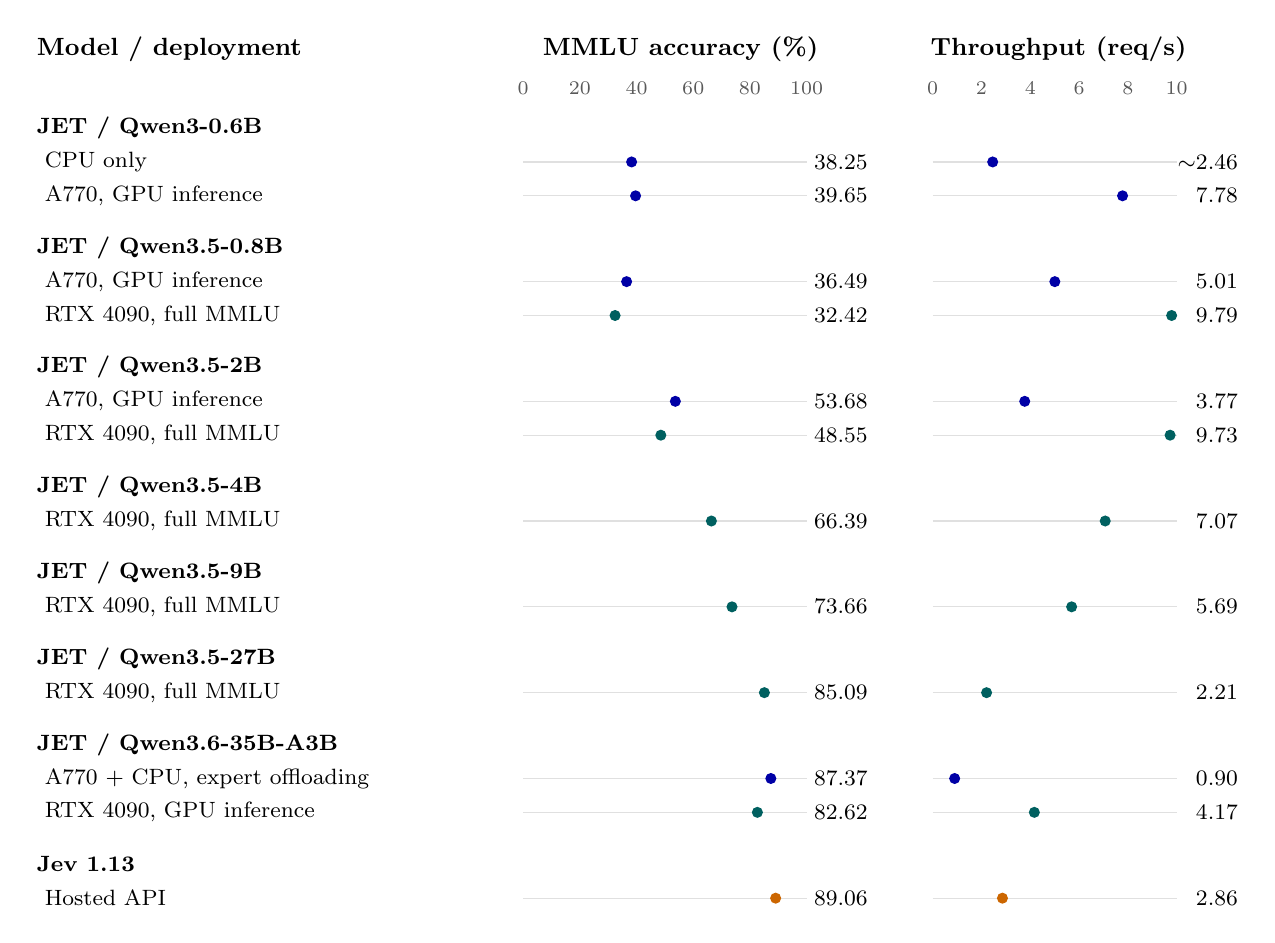
\begin{tikzpicture}[x=1cm,y=1cm,font=\footnotesize]
\node[anchor=west,font=\small\bfseries] at (0,0.8) {Model / deployment};
\node[font=\small\bfseries] at (8.3,0.8) {MMLU accuracy (\%)};
\node[font=\small\bfseries] at (13.1,0.8) {Throughput (req/s)};
\node[font=\scriptsize,text=black!65] at (6.3,0.3) {0};
\node[font=\scriptsize,text=black!65] at (7.02,0.3) {20};
\node[font=\scriptsize,text=black!65] at (7.74,0.3) {40};
\node[font=\scriptsize,text=black!65] at (8.46,0.3) {60};
\node[font=\scriptsize,text=black!65] at (9.18,0.3) {80};
\node[font=\scriptsize,text=black!65] at (9.9,0.3) {100};
\node[font=\scriptsize,text=black!65] at (11.5,0.3) {0};
\node[font=\scriptsize,text=black!65] at (12.12,0.3) {2};
\node[font=\scriptsize,text=black!65] at (12.74,0.3) {4};
\node[font=\scriptsize,text=black!65] at (13.36,0.3) {6};
\node[font=\scriptsize,text=black!65] at (13.98,0.3) {8};
\node[font=\scriptsize,text=black!65] at (14.6,0.3) {10};
\node[anchor=west,font=\footnotesize\bfseries] at (0,-0.2) {JET / Qwen3-0.6B};
\node[anchor=west] at (0.1,-0.63) {CPU only};
\draw[black!12] (6.3,-0.63) -- (9.9,-0.63);
\draw[black!12] (11.5,-0.63) -- (14.6,-0.63);
\fill[blue!65!black] (7.6770,-0.63) circle (2pt);
\node[anchor=east] at (10.8,-0.63) {38.25};
\fill[blue!65!black] (12.2626,-0.63) circle (2pt);
\node[anchor=east] at (15.5,-0.63) {\(\sim\)2.46};
\node[anchor=west] at (0.1,-1.06) {A770, GPU inference};
\draw[black!12] (6.3,-1.06) -- (9.9,-1.06);
\draw[black!12] (11.5,-1.06) -- (14.6,-1.06);
\fill[blue!65!black] (7.7274,-1.06) circle (2pt);
\node[anchor=east] at (10.8,-1.06) {39.65};
\fill[blue!65!black] (13.9118,-1.06) circle (2pt);
\node[anchor=east] at (15.5,-1.06) {7.78};
\node[anchor=west,font=\footnotesize\bfseries] at (0,-1.72) {JET / Qwen3.5-0.8B};
\node[anchor=west] at (0.1,-2.15) {A770, GPU inference};
\draw[black!12] (6.3,-2.15) -- (9.9,-2.15);
\draw[black!12] (11.5,-2.15) -- (14.6,-2.15);
\fill[blue!65!black] (7.6136,-2.15) circle (2pt);
\node[anchor=east] at (10.8,-2.15) {36.49};
\fill[blue!65!black] (13.0520,-2.15) circle (2pt);
\node[anchor=east] at (15.5,-2.15) {5.01};
\node[anchor=west] at (0.1,-2.58) {RTX 4090, full MMLU};
\draw[black!12] (6.3,-2.58) -- (9.9,-2.58);
\draw[black!12] (11.5,-2.58) -- (14.6,-2.58);
\fill[teal!75!black] (7.4670,-2.58) circle (2pt);
\node[anchor=east] at (10.8,-2.58) {32.42};
\fill[teal!75!black] (14.5352,-2.58) circle (2pt);
\node[anchor=east] at (15.5,-2.58) {9.79};
\node[anchor=west,font=\footnotesize\bfseries] at (0,-3.24) {JET / Qwen3.5-2B};
\node[anchor=west] at (0.1,-3.6700000000000004) {A770, GPU inference};
\draw[black!12] (6.3,-3.6700000000000004) -- (9.9,-3.6700000000000004);
\draw[black!12] (11.5,-3.6700000000000004) -- (14.6,-3.6700000000000004);
\fill[blue!65!black] (8.2325,-3.6700000000000004) circle (2pt);
\node[anchor=east] at (10.8,-3.6700000000000004) {53.68};
\fill[blue!65!black] (12.6694,-3.6700000000000004) circle (2pt);
\node[anchor=east] at (15.5,-3.6700000000000004) {3.77};
\node[anchor=west] at (0.1,-4.1000000000000005) {RTX 4090, full MMLU};
\draw[black!12] (6.3,-4.1000000000000005) -- (9.9,-4.1000000000000005);
\draw[black!12] (11.5,-4.1000000000000005) -- (14.6,-4.1000000000000005);
\fill[teal!75!black] (8.0480,-4.1000000000000005) circle (2pt);
\node[anchor=east] at (10.8,-4.1000000000000005) {48.55};
\fill[teal!75!black] (14.5157,-4.1000000000000005) circle (2pt);
\node[anchor=east] at (15.5,-4.1000000000000005) {9.73};
\node[anchor=west,font=\footnotesize\bfseries] at (0,-4.760000000000001) {JET / Qwen3.5-4B};
\node[anchor=west] at (0.1,-5.19) {RTX 4090, full MMLU};
\draw[black!12] (6.3,-5.19) -- (9.9,-5.19);
\draw[black!12] (11.5,-5.19) -- (14.6,-5.19);
\fill[teal!75!black] (8.6902,-5.19) circle (2pt);
\node[anchor=east] at (10.8,-5.19) {66.39};
\fill[teal!75!black] (13.6917,-5.19) circle (2pt);
\node[anchor=east] at (15.5,-5.19) {7.07};
\node[anchor=west,font=\footnotesize\bfseries] at (0,-5.8500000000000005) {JET / Qwen3.5-9B};
\node[anchor=west] at (0.1,-6.28) {RTX 4090, full MMLU};
\draw[black!12] (6.3,-6.28) -- (9.9,-6.28);
\draw[black!12] (11.5,-6.28) -- (14.6,-6.28);
\fill[teal!75!black] (8.9519,-6.28) circle (2pt);
\node[anchor=east] at (10.8,-6.28) {73.66};
\fill[teal!75!black] (13.2651,-6.28) circle (2pt);
\node[anchor=east] at (15.5,-6.28) {5.69};
\node[anchor=west,font=\footnotesize\bfseries] at (0,-6.94) {JET / Qwen3.5-27B};
\node[anchor=west] at (0.1,-7.37) {RTX 4090, full MMLU};
\draw[black!12] (6.3,-7.37) -- (9.9,-7.37);
\draw[black!12] (11.5,-7.37) -- (14.6,-7.37);
\fill[teal!75!black] (9.3632,-7.37) circle (2pt);
\node[anchor=east] at (10.8,-7.37) {85.09};
\fill[teal!75!black] (12.1851,-7.37) circle (2pt);
\node[anchor=east] at (15.5,-7.37) {2.21};
\node[anchor=west,font=\footnotesize\bfseries] at (0,-8.03) {JET / Qwen3.6-35B-A3B};
\node[anchor=west] at (0.1,-8.459999999999999) {A770 + CPU, expert offloading};
\draw[black!12] (6.3,-8.459999999999999) -- (9.9,-8.459999999999999);
\draw[black!12] (11.5,-8.459999999999999) -- (14.6,-8.459999999999999);
\fill[blue!65!black] (9.4453,-8.459999999999999) circle (2pt);
\node[anchor=east] at (10.8,-8.459999999999999) {87.37};
\fill[blue!65!black] (11.7795,-8.459999999999999) circle (2pt);
\node[anchor=east] at (15.5,-8.459999999999999) {0.90};
\node[anchor=west] at (0.1,-8.889999999999999) {RTX 4090, GPU inference};
\draw[black!12] (6.3,-8.889999999999999) -- (9.9,-8.889999999999999);
\draw[black!12] (11.5,-8.889999999999999) -- (14.6,-8.889999999999999);
\fill[teal!75!black] (9.2742,-8.889999999999999) circle (2pt);
\node[anchor=east] at (10.8,-8.889999999999999) {82.62};
\fill[teal!75!black] (12.7915,-8.889999999999999) circle (2pt);
\node[anchor=east] at (15.5,-8.889999999999999) {4.17};
\node[anchor=west,font=\footnotesize\bfseries] at (0,-9.549999999999999) {Jev 1.13};
\node[anchor=west] at (0.1,-9.979999999999999) {Hosted API};
\draw[black!12] (6.3,-9.979999999999999) -- (9.9,-9.979999999999999);
\draw[black!12] (11.5,-9.979999999999999) -- (14.6,-9.979999999999999);
\fill[orange!80!black] (9.5062,-9.979999999999999) circle (2pt);
\node[anchor=east] at (10.8,-9.979999999999999) {89.06};
\fill[orange!80!black] (12.3866,-9.979999999999999) circle (2pt);
\node[anchor=east] at (15.5,-9.979999999999999) {2.86};
\end{tikzpicture}
\caption{MMLU accuracy and throughput for selected JET configurations with reasoning disabled, and Jev 1.13. Blue: CPU/Arc A770; teal: RTX 4090; orange: hosted API. A770 expert offloading executes some model experts on CPU. JET CPU/A770 accuracy uses an MMLU subset and throughput covers the mixed BoolQ/MMLU workload. RTX 4090 accuracy and throughput come from the same full-MMLU run for each model. Jev uses full-MMLU accuracy and a separately reported API rate. Each metric uses a common horizontal scale.}
\label{fig:mmlu-throughput}
\end{figure}


Each displayed JET point combines accuracy and throughput from the same
complete full-MMLU run. Section~\ref{sec:finetuning} describes the separately
marked LoRA adaptation. No partial run or pending Arc A770 result supplies
a point. External model-card results have no corresponding JET throughput.

\subsection{Reference Comparison with Larger Models and Jev}
The author's manual Jev 1.13 measurement is 89.06\% on full MMLU,
with a separately reported API rate of 2.86 requests/s. Its evaluated interface
is sampler-free and exposes no configurable reasoning or few-shot settings.
These are the author's measurements, not provider-published results.
Published larger-model scores retain their source protocols.

\begin{table}[htbp]
\centering\small
\caption{MMLU reference comparison. Protocols differ; this is numerical
context rather than a matched ranking. External models were not run in JET.}
\label{tab:mmlu-comparison}
\begin{tabular}{>{\raggedright\arraybackslash}p{6.0cm}r>{\raggedright\arraybackslash}p{6.2cm}}
\toprule
System / model & MMLU (\%) & Evaluation basis \\
\midrule
\multicolumn{3}{l}{\emph{Full-MMLU evaluations}} \\
JET / Qwen3.5-27B, RTX 4090 & \jetresult{full-27b-vulkan}{accuracy} & Mean-token scoring; Vulkan; local execution \\
JET / Qwen3.6-35B-A3B, RTX 4090 & \jetresult{full-35b-vulkan}{accuracy} & Mean-token scoring; Vulkan; local execution \\
Jev 1.13 & 89.06 & Native decision interface \\
\midrule
\multicolumn{3}{l}{\emph{Published larger-model references}} \\
Llama 3.1 70B Instruct~\cite{llama31-card} & 83.6 & 5-shot; subject-macro accuracy \\
Llama 3.1 405B Instruct~\cite{llama31-card} & 87.3 & 5-shot; subject-macro accuracy \\
Qwen2.5-72B-Instruct~\cite{deepseek-v3-results} & 85.3 & MMLU exact match in the cited comparison \\
DeepSeek-V3 (671B)~\cite{deepseek-v3-results} & 88.5 & MMLU exact match in the cited comparison \\
\bottomrule
\end{tabular}
\end{table}

The highest measured JET configuration is \jetresult{best}{model}, with
\jetresult{best}{accuracy}\% accuracy. The signed Jev-minus-JET difference
is \jetresult{best}{gap-to-jev} percentage points. Shared benchmark coverage
does not imply identical prompting, scoring, aggregation, or statistical
equivalence. Likewise, local complete-process throughput and an API rate with
undocumented concurrency do not support a controlled speedup claim.

Both systems provide sampler-free decisions over supplied alternatives.
JET returns normalized decision weights for named choices and computes ordinal
scores as expectations of zero-based level indices. Jev additionally reports
separate confidence values; JET's weights are not equivalent calibrated
confidence estimates. Jev describes parallel evaluation of independent
questions, whereas JET's hybrid path evaluates candidate continuations serially
with a shared prefix~\cite{jev-docs,jev-workflows}.

\subsection{Shared-Prefix Execution: Pending Follow-Up}
\label{sec:prefix-results}
The Arc A770 follow-up will compare independent candidate execution with
prefix reuse and metadata-only cache resets under the same mean-token rule.
The fixed workload comprises 256 BoolQ validation examples and five MMLU
test examples from each subject, totaling 541 requests~\cite{boolq,mmlu}.
Speedup, prefix-token counts, and exact-response equivalence require new
measurements. Earlier execution measurements do not establish those properties
for the method evaluated here.

\subsection{Numerical Equivalence and Reproducibility}
\label{sec:repeatability}
Sampler-free selection does not ensure agreement across numerical backends.
The current control suite compares paired answers and decision weights, including
fresh-process repetitions of the smallest model. Independent candidate execution
provides a reference for state-isolation testing. Numerical claims about prefix
reuse and independent-request batching remain pending under the current method;
the production hybrid path retains serial candidate continuations.
